\documentclass[UTF8,openany]{ctexbook}

% 论文版面要求:
% 统一按 word 格式A4纸(页面设置按word默认值)编排、打印、制作。
% 正文内容字体为宋体;字号为小4号;字符间距为标准;行距为25磅(约0.88175cm)。

%%%%% ===== 页面设置
\usepackage[a4paper,top=2.54cm,bottom=2.54cm,left=3.17cm,right=3.17cm,%
            ]{geometry}
\usepackage{tcolorbox}
\usepackage{colortbl}
\usepackage{dirtree}
\usepackage{longtable}
\usepackage{booktabs}
            
\setlength{\parindent}{2em}
%默认的弹性间距会导致文中某些排版flush的时候,出现大量空白。
\setlength{\parskip}{0.5em} %指定固定段后间距,默认为弹性间距。
\setlength{\intextsep}{10pt} %固定浮浮动体前后间距。
\usepackage{enumitem}
\usepackage{ulem}

%%%%% =====章节 标题 设置
\ctexset{%
  contentsname={\vspace{-3.5em}\centerline{\zihao{-3}\heiti 目\quad 录}\vspace{-0.7em}},
  listfigurename={\vspace{-3.5em}\centerline{\zihao{-3}\heiti 插\ 图\ 目\ 录}\vspace{-0.5em}},
  listtablename={\vspace{-3.5em}\centerline{\zihao{-3}\heiti 表\ 格\ 目\ 录}\vspace{-0.5em}},
  bibname={\vspace{-3em}\centerline{\zihao{-3}\heiti 参\ 考\ 文\ 献}\vspace{3em}},
  chapter={name={,},
  number=\arabic{chapter}, %指定章序号为一二三。。。。
  nameformat={\zihao{-2}\bfseries},
  titleformat={\zihao{-2}\bfseries},
  format=\raggedright,
  beforeskip={10pt},
  afterskip={10pt},
  pagestyle={fancy}
  },
section={format=\raggedright,
  nameformat={\zihao{4}\bfseries},
  titleformat={\zihao{4}\bfseries},
%           afterskip={1ex plus 0.2ex}
  beforeskip={1ex},% 固定段前段后间距,
  afterskip={1ex}
  },
subsection={format=\raggedright,
  nameformat={\zihao{-4}\bfseries},
  titleformat={\zihao{-4}\bfseries},
%           afterskip={0.5ex plus 0.1ex}
  beforeskip={0.5ex},
  afterskip={0.5ex}
  }
}
%%%%% ===== 中英文字体
%\setsansfont{Myriad Pro} % 无衬线字体 sans serif \sffamily
%\setmonofont{Consolas}   % 等宽字体 typewriter \ttfamily
%\newcommand{\Times}{\fontspec{Times New Roman}}
%% 中文字体
%\setCJKmainfont[BoldFont={Microsoft YaHei},ItalicFont={KaiTi}]{NSimSun}
%\setCJKsansfont{Microsoft YaHei}
%\setCJKmonofont{KaiTi}
%\setCJKfamilyfont{STSong}{方正小标宋_GBK}\newcommand{\STSong}{\CJKfamily{STSong}}
\setCJKfamilyfont{songti}{STZhongsong}\newcommand{\STSong}{\CJKfamily{STSong}}

%%%%% ===== 常用宏包
\usepackage{amsmath,amssymb,amsfonts,bm}
\usepackage[amsmath,thref,thmmarks,hyperref]{ntheorem}
\usepackage{graphicx,xcolor,float}
\usepackage{fancyhdr}
\usepackage{tocloft} % 设置目录中的条目间距


\renewcommand\cftdot{\textsubscript{……}}
\renewcommand\cftdotsep{0}

\setlength{\cftbeforechapskip}{1pt}
\renewcommand{\cftchapleader}{\cftdotfill{\cdot}}


\usepackage{booktabs} % toprule, midrule, bottomrule
\usepackage{varwidth} % 可变宽度的 parbox

% %%%%% ===== 参考文献与链接
% \usepackage[numbers,sort&compress,sectionbib,super, square]{natbib} %引用上标,禁用连续缩写。
% \newcommand{\upcite}[1]{\textsuperscript{\cite{#1}}}


\usepackage[xetex,pagebackref]{hyperref}
\hypersetup{CJKbookmarks=true,colorlinks=true,citecolor=blue,%
            linkcolor=blue,urlcolor=blue,bookmarksnumbered=true,%
	        bookmarksopen=true,breaklinks=true}
	        
	        
	        
\iffalse   % 调试时,可去掉,以用于显示引用位置。
\renewcommand*{\backrefalt}[4]{%
\ifcase #1 No citations.%
\or Cited on page #2.%
\else Cited on pages #2.%
%\else #1 Cited on pages #2.%
\fi
}

\else
\renewcommand*{\backrefalt}[4]{}
\fi

%%%%% ===== 浮动图表的标题
\usepackage[margin=2em,labelsep=space,skip=0.5em,font=normalfont]{caption}
\DeclareCaptionFormat{mycaption}{{\heiti\color{blue} #1}#2{\kaishu #3}}
\captionsetup{format=mycaption,tablewithin=chapter,figurewithin=chapter}%,belowskip=-10pt
%\setlength{\belowcaptionskip}{-10pt}

%%%%%% ===== 浮动图表的比例默认50%以下,否则无法浮动。
\renewcommand\floatpagefraction{.9} %当浮动体小于页面90%时进行直接放置。
\renewcommand\topfraction{.9}  
\renewcommand\bottomfraction{.9}  
\renewcommand\textfraction{.1}



%%%%% ===== 算法
\usepackage{algorithm,algpseudocode}

%%%%% ===== 其他
\usepackage{ulem}
\def\ULthickness{1pt}




%%%%%===== Code Style代码
\usepackage{listings}
\usepackage{color}

\definecolor{dkgreen}{rgb}{0,0.6,0}
\definecolor{gray}{rgb}{0.5,0.5,0.5}
\definecolor{mauve}{rgb}{0.58,0,0.82}

\usepackage{accsupp}



\newcommand\emptyaccsupp[1]{\BeginAccSupp{ActualText={}}#1\EndAccSupp{}}

\lstset{
    % language = C,
    showstringspaces=false,
    xleftmargin = 3em,xrightmargin = 3em, aboveskip = 1em,
	backgroundcolor = \color{white}, % 背景色
	basicstyle = \small\ttfamily, % 基本样式 + 小号字体
	rulesepcolor= \color{gray}, % 代码块边框颜色
	breaklines = true, % 代码过长则换行
	numbers = left, % 行号在左侧显示
	numberstyle=\emptyaccsupp,
    numbersep = 14pt, 
    keywordstyle=\color{purple}\bfseries, % 关键字颜色
    commentstyle =\color{red!50!green!50!blue!60}, % 注释颜色
    stringstyle = \color{red}, % 字符串颜色
    morekeywords={ASSERT, int64_t, uint32_t},
	% frame = shadowbox, % 用(带影子效果)方框框住代码块
	frame = single, % 用(带影子效果)方框框住代码块
	showspaces = false, % 不显示空格
	columns = fixed, % 字间距固定
  framesep=1em
} 
\lstset{
    sensitive=true,
    moreemph={ASSERT, NULL}, emphstyle=\color{red}\bfseries,
    moreemph=[2]{int64_t, uint32_t, tid_t, uint8_t, int16_t, uint16_t, int32_t, size_t}, emphstyle=[2]\color{purple}\bfseries,
    showspaces = false, % 不显示空格
    }



\newcommand{\mcc}[1]{\multicolumn{1}{c}{\underline{\makebox[10em][c]{#1}}}}
\newcommand{\mce}[1]{\multicolumn{1}{c}{\underline{\makebox[15em][l]{#1}}}}


\pagestyle{fancy}
\fancyhf{}  % 清除以前对页眉页脚的设置

\newcommand{\makeheadrule}{%% 定义页眉与正文间双隔线
    \makebox[0pt][l]{\rule[.7\baselineskip]{\headwidth}{0.3pt}}%0.4
    \rule[0.85\baselineskip]{\headwidth}{1.0pt}\vskip-.8\baselineskip}
\makeatletter
\renewcommand{\headrule}{%
    % {\if@fancyplain\let\headrulewidth\plainheadrulewidth\fi\makeheadrule}}
    {\makeheadrule}}
\makeatother
\renewcommand{\chaptermark}[1]{\markboth{\CTEXthechapter \ #1}{}}
\renewcommand{\sectionmark}[1]{\markright{\thesection \ #1}{}}
%\fancyhead[RO,LE]{{\small\songti\rightmark}}     % 节标题
%\fancyhead[RE]{{\small\songti\leftmark}}      % 章标题
\fancyhead[L]{《数据库系统及应用实践》课程项目报告}
\fancyhead[R]{COVIDLIT SEARCH}
% \fancyhead[RO,LE]{$\cdot$ {\small\thepage} $\cdot$}
\fancyfoot[C]{{-\thepage-}}
%\fancyfoot[CO,CE]{{\thepage}}

\ctexset{chapter/break={}}

\begin{document}

\begin{titlepage}
    \begin{center}

        % {
        %     \begin{figure}[H]
        %         \vspace{5cm}
        %         
\includegraphics[width=14cm]{img/0.png}
        %     \end{figure}
        %     \heiti\zihao{2}《数据库系统及应用实践》课程项目报告\\
        %     \vspace{0.8em}
        %     \zihao{2}\textbf{CovidLit Search}\Large{(Milestone 2)}
        % }
        % \\[10em]
        \zihao{-3}
        \begin{tabular}{p{0cm}p{5.5em}@{\extracolsep{0.5ex}}cc}
            ~ & \hfill 小\ 组\ 成\ 员: &  & \mcc{李鹏达\quad 10225101460}      \\
            ~ & \hfill             &  & \mcc{武泽恺\quad 10225101429}      \\
            ~ & \hfill             &  & \mcc{王\quad 力\quad 10225101434} \\
        \end{tabular}
        \\[8em]
        \zihao{-2}2024年5月 - 6月
    \end{center}
    \thispagestyle{fancy}
    \fancyfoot[C]{}
\end{titlepage}
\fancyfoot[C]{-\thepage-}

\setcounter{page}{1}
\pagenumbering{roman}
\tableofcontents
\thispagestyle{fancy}
\newpage

\setcounter{page}{1}
\pagenumbering{arabic}

\chapter{项目简介}

本项目(“CovidLit Search”)致力于为研究人员提供一个方便的、用户友好的COVID-19相关文献检索工具,以帮助他们更快地找到相关文献进行参考研究。

本项目的目标是通过提供一个简单友好的界面,使用户能够快速搜索到与COVID-19相关的文献,并且能够根据作者、时间和期刊等信息进行检索。此外,本项目也允许用户通过研究方向、研究对象和研究问题等信息准确检索部分文献并对其他文献进行模糊搜索,以便用户查找到最相关的文献。

另外,本项目还提供了一个用户注册和登录系统。用户可以通过注册登录后,将自己的搜索历史保存在云端,以便在不同设备上查看自己的搜索历史。用户还可以将自己感兴趣的文献加入到自己的收藏夹中或订阅期刊,以便在以后查看。

本项目名称为 ``CovidLit Search'',意为 ``COVID-19 Literature Search'',即 COVID-19 相关文献检索。

\chapter{数据库设计}

\section{概述}
\label{sec:overviewOfDatabaseDesign}

为了实现文献检索系统,我们需要设计一个数据库来存储文献、期刊、作者和引用等信息。

为了实现相关功能,我们考虑使用 Entity-Relation 模型来设计数据库。我们考虑设计文章(article)、作者(author)、期刊(journal)和用户(user)等实体集,以及撰写(write)、引用(cite)、订阅(subscribe)、收藏(collect)和浏览历史(history)等联系集。

其中,文章(article)与作者(author)通过撰写(write)联系集相连,表示作者撰写了文章;文章(article)与期刊(journal)通过发表(publish)联系集相连,表示文章在期刊上发表;文章(article)与文章(article)通过引用(cite)联系集相连,标识不同文章之间的引用与被引用关系;用户(user)与文章(article)通过收藏(collect)浏览历史(history)联系集相连,表示用户收藏了文章和用户的历史浏览文章;用户(user)与期刊(journal)通过订阅(subscribe)联系集相连,表示作者订阅了该期刊,可能希望获取该期刊的最新文章。

起初,我们考虑使用 MySQL 数据库来存储数据,并成功地将小数据集的数据导入了数据库中,完成了基本的测试。但在完成实验5后,我们发现 PostgreSQL 在多表的复杂查询上的性能要明显优于 MySQL,在数据规模较大的完整数据集上,PostgreSQL 的性能可能会更优。因此,我们决定改用 PostgreSQL 数据库来存储数据。

\section{表结构}

\subsection{实体集}

用户(user)表存储用户的基本信息,其结构如下:

\begin{table}[H]
    \centering
    \begin{tabular}{|c|c|c|c|c|}
        \hline
        \textbf{字段名} & \textbf{类型} & \textbf{主键} & \textbf{外键} & \textbf{说明} \\
        \hline
        \textit{id} & \texttt{INT} & 是 &  & 用户ID,自动递增 \\
        \hline
        \textit{nickname} & \texttt{VARCHAR(100)} &  &  & 用户名(昵称) \\
        \hline
        \textit{email} & \texttt{VARCHAR(200)} &  &  & 邮箱 \\
        \hline
        \textit{password} & \texttt{VARCHAR(100)} &  &  & 密码(加密后) \\
        \hline
        \textit{avatar} & \texttt{VARCHAR(500)} &  &  & 头像 \\
        \hline
        \textit{motto} & \texttt{VARCHAR(1000)} &  &  & 座右铭 \\
        \hline
        \textit{collage} & \texttt{VARCHAR(100)} &  &  & 学院(学校) \\
        \hline
        \textit{subscribe\_email} & \texttt{BOOLEAN} &  &  & 是否订阅邮件 \\
        \hline
        \textit{save\_history} & \texttt{BOOLEAN} &  &  & 是否保存历史记录 \\
        \hline
    \end{tabular}
    \caption{用户(\textit{user})表}
\end{table}

文章(article)表存储文章的基本信息,其结构如下:

\begin{table}[H]
    \centering
    \begin{tabular}{|c|c|c|c|c|}
        \hline
        \textbf{字段名} & \textbf{类型} & \textbf{主键} & \textbf{外键} & \textbf{说明} \\
        \hline
        \textit{id} & \texttt{VARCHAR(50)} & 是 &  & 文章ID \\
        \hline
        \textit{title} & \texttt{VARCHAR(1000)} &  &  & 文章标题 \\
        \hline
        \textit{abstract} & \texttt{TEXT} &  &  & 摘要 \\
        \hline
        \textit{doi} & \texttt{VARCHAR(50)} &  &  & 数字对象唯一标识符 \\
        \hline
        \textit{license} & \texttt{VARCHAR(50)} &  &  & 许可 \\
        \hline
        \textit{publish\_time} & \texttt{DATETIME} &  &  & 发表时间 \\
        \hline
        \textit{url} & \texttt{VARCHAR(800)} &  &  & 文章URL \\
        \hline
        \textit{study\_type} & \texttt{VARCHAR(500)} &  &  & 研究类型 \\
        \hline
        \textit{addressed\_population} & \texttt{VARCHAR(1000)} &  &  & 研究对象人群 \\
        \hline
        \textit{challenge} & \texttt{VARCHAR(2000)} &  &  & 挑战/研究问题 \\
        \hline
        \textit{focus} & \texttt{VARCHAR(100)} &  &  & 研究重点 \\
        \hline
    \end{tabular}
    \caption{文章(\textit{article})表}
\end{table}

期刊(journal)表存储期刊的基本信息,其结构如下:

\begin{table}[H]
    \centering
    \begin{tabular}{|c|c|c|c|c|}
        \hline
        \textbf{字段名} & \textbf{类型} & \textbf{主键} & \textbf{外键} & \textbf{说明} \\
        \hline
        \textit{name} & \texttt{VARCHAR(100)} & 是 &  & 期刊名称 \\
        \hline
        \textit{description} & \texttt{VARCHAR(1000)} &  &  & 期刊描述 \\
        \hline
    \end{tabular}
    \caption{期刊(\textit{journal})表}
\end{table}

作者(author)表存储作者的基本信息,其结构如下:

\begin{table}[H]
    \centering
    \begin{tabular}{|c|c|c|c|c|}
        \hline
        \textbf{字段名} & \textbf{类型} & \textbf{主键} & \textbf{外键} & \textbf{说明} \\
        \hline
        \textit{name} & \texttt{VARCHAR(100)} & 是 &  & 作者姓名 \\
        \hline
        \textit{email} & \texttt{VARCHAR(1000)} &  &  & 邮箱 \\
        \hline
        \textit{lab} & \texttt{VARCHAR(1000)} &  &  & 所在实验室 \\
        \hline
        \textit{institution} & \texttt{VARCHAR(1000)} &  &  & 所在机构 \\
        \hline
        \textit{country} & \texttt{VARCHAR(100)} &  &  & 国家 \\
        \hline
        \textit{post\_code} & \texttt{VARCHAR(100)} &  &  & 邮政编码 \\
        \hline
        \textit{settlement} & \texttt{VARCHAR(100)} &  &  & 定居点(城市) \\
        \hline
    \end{tabular}
    \caption{作者(\textit{author})表}
\end{table}

\subsection{联系集}

撰写(write)联系集存储文章与作者之间的联系,其结构如下:

\begin{table}[H]
    \centering
    \begin{tabular}{|c|c|c|c|c|}
        \hline
        \textbf{字段名} & \textbf{类型} & \textbf{主键} & \textbf{外键} & \textbf{说明} \\
        \hline
        \textit{author\_name} & \texttt{VARCHAR(100)} & 是 & \textit{author(name)} & 作者姓名 \\
        \hline
        \textit{article\_id} & \texttt{VARCHAR(50)} & 是 & \textit{article(id)} & 文章ID \\
        \hline
    \end{tabular}
    \caption{撰写关系(\textit{write})表}
\end{table}

发表(publish)联系集存储文章与期刊之间的联系,其结构如下:

\begin{table}[H]
    \centering
    \begin{tabular}{|c|c|c|c|c|}
    \hline
    \textbf{字段名} & \textbf{类型} & \textbf{主键} & \textbf{外键} & \textbf{说明} \\
    \hline
    \textit{journal\_name} & \texttt{VARCHAR(100)} & 是 & \textit{journal(name)} & 期刊名称 \\
    \hline
    \textit{article\_id} & \texttt{VARCHAR(50)} & 是 & \textit{article(id)} & 文章ID \\
    \hline
    \textit{volume} & \texttt{VARCHAR(50)} & & & 卷号 \\
    \hline
    \textit{pages} & \texttt{VARCHAR(200)} & & & 页码 \\
    \hline
    \end{tabular}
    \caption{发表关系(\textit{publish})表}
\end{table}


引用(cite)联系集存储文章与文章之间的引用关系,其结构如下:

\begin{table}[H]
    \centering
    \begin{tabular}{|c|c|c|c|c|}
        \hline
        \textbf{字段名} & \textbf{类型} & \textbf{主键} & \textbf{外键} & \textbf{说明} \\
        \hline
        \textit{citing\_id} & \texttt{VARCHAR(100)} & 是 & \textit{article(id)} & 引用文章ID \\
        \hline
        \textit{cited\_id} & \texttt{VARCHAR(100)} & 是 & \textit{article(id)} & 被引用文章ID \\
        \hline
    \end{tabular}
    \caption{引用关系(\textit{cite})表}
\end{table}

收藏(collect)联系集存储用户与文章之间的收藏关系,其结构如下:

\begin{table}[H]
    \centering
    \begin{tabular}{|c|c|c|c|c|}
        \hline
        \textbf{字段名} & \textbf{类型} & \textbf{主键} & \textbf{外键} & \textbf{说明} \\
        \hline
        \textit{user\_id} & \texttt{INT} & 是 & \textit{user(id)} & 用户ID \\
        \hline
        \textit{article\_id} & \texttt{VARCHAR(50)} & 是 & \textit{article(id)} & 文章ID \\
        \hline
    \end{tabular}
    \caption{收藏关系(\textit{collect})表}
\end{table}

订阅(subscribe)联系集存储用户与期刊之间的订阅关系,其结构如下:

\begin{table}[H]
    \centering
    \begin{tabular}{|c|c|c|c|c|}
        \hline
        \textbf{字段名} & \textbf{类型} & \textbf{主键} & \textbf{外键} & \textbf{说明} \\
        \hline
        \textit{user\_id} & \texttt{INT} & 是 & \textit{user(id)} & 用户ID \\
        \hline
        \textit{journal\_name} & \texttt{VARCHAR(200)} & 是 & \textit{journal(name)} & 期刊名称 \\
        \hline
    \end{tabular}
    \caption{订阅关系(\textit{subscribe})表}
\end{table}

浏览历史(history)联系集存储用户与文章之间的浏览历史关系,其结构如下:

\begin{table}[H]
    \centering
    \begin{tabular}{|c|c|c|c|c|}
        \hline
        \textbf{字段名} & \textbf{类型} & \textbf{主键} & \textbf{外键} & \textbf{说明} \\
        \hline
        \textit{user\_id} & \texttt{INT} & 是 & \textit{user(id)} & 用户ID \\
        \hline
        \textit{article\_id} & \texttt{VARCHAR(50)} & 是 & \textit{article(id)} & 文章ID \\
        \hline
        \textit{time} & \texttt{DATETIME} & 是 &  & 浏览时间 \\
        \hline
    \end{tabular}
    \caption{浏览历史(\textit{history})表}
\end{table}

\section{E-R 图}


根据上述设计,我们绘制了数据库的 E-R 图,如图 \ref{fig:er} 所示。

% \begin{figure}[H]
%     \centering
%     \includegraphics[width=0.9\textwidth]{img/ER.png}
%     \caption{数据库 E-R 图}
%     \label{fig:er}
% \end{figure}

其中,PK 表示主键,FK 表示外键。

\section{\texttt{schema}}

根据上述设计,我们可以写出数据库的 \texttt{schema},如下所示:

\begin{tcolorbox}
    \raggedright
    \hangafter=1
    \hangindent=3em
    \it
    article(\uline{id}, title, abstract, doi, license, publish\_time, url, study\_type, addressed\_population,
    challenge, focus)

    author(\uline{name}, email, lab, institution, country, post\_code, settlement)

    write(\uline{author\_name}, \uline{article\_id})

    journal(\uline{name}, description)

    publish(\uline{journal\_name}, \uline{article\_id}, volume, pages)

    cite(\uline{citing\_id}, \uline{cited\_id})

    \hangafter=1
    \hangindent=2em
    user(\uline{id}, nickname, email, password, avatar, motto, collage, subscribe\_email, save\_history)

    collect(\uline{user\_id}, \uline{article\_id})

    subscribe(\uline{user\_id}, \uline{journal\_name})

    history(\uline{user\_id}, \uline{article\_id}, time)
\end{tcolorbox}



\chapter{数据集}

\section{数据来源}

本项目使用的数据集是由美国白宫联合一系列顶尖研究机构提供的COVID-19 Open Research Dataset (CORD-19)。该数据集可以在Kaggle上下载\footnote{\url{https://www.kaggle.com/datasets/allen-institute-for-ai/CORD-19-research-challenge}},它包含了超过1,000,000篇来自PubMed、PMC、bioRxiv和medRxiv等来源的COVID-19相关文献的元数据,其中400,000篇提供全文。此外,该数据集还包括超过 6,000篇按研究方向分类的文献元数据,包括研究方向、研究对象和研究问题等信息。

该数据集的元数据包括文献标题、作者、摘要、发布时间、期刊、全文链接等信息。我们将使用这些信息来构建我们的文献检索系统。


\section{数据处理}

\subsection{数据集结构}

我们首先对数据集进行了初步的探索,其结构如图 \ref{fig:dataset} 所示。数据集主要包括以下几个部分:

\begin{enumerate}
    \item \texttt{metadata.csv}:包含了文献的元数据,包括文献标题、作者、摘要、发布时间、期刊、全文链接等信息。
    \item \texttt{metadata.readme}:包含数据集内容的更新日志。
    \item \texttt{json\_schema.txt}:包含了数据集中的\texttt{JSON}文件的结构。
    \item \texttt{COVID.DATA.LIC.AGMT.pdf}:包含了数据集的使用许可协议。
    \item \texttt{document\_parses/}:文件夹,包含了数据集中的文献全文,以\texttt{JSON}格式存储。
    \item \texttt{Kaggle/target\_tables/}:文件夹,包含了数据集中的研究方向分类的文献元数据,包括研究方向、研究对象和研究问题等信息。
    \item \texttt{cord\_19\_embeddings/}:文件夹,包含了数据集中的文献的嵌入向量。

\end{enumerate}
% \begin{figure}[H]
%     \dirtree{%
%         .1 archive.
%         .2 metadata.csv\DTcomment{1}.
%         .2 metadata.readme\DTcomment{2}.
%         .2 json\_schema.txt\DTcomment{3}.
%         .2 COVID.DATA.LIC.AGMT.pdf\DTcomment{4}.
%         .2 document\_parses\DTcomment{5}.
%         .3 pdf\_json.
%         .4 $\cdots$ .
%         .3 pmc\_json.
%         .4 $\cdots$ .
%         .2 Kaggle.
%         .3 target\_tables\DTcomment{6}.
%         .4 0\_table\_formats\_and\_column\_definitions.
%         .4 1\_population.
%         .5 $\cdots$ .
%         .4 $\cdots$.
%         .3 cord\_19\_embeddings\DTcomment{7}.
%         .4 cord\_19\_embeddings-2022-06-02.csv.
%     }
%     \caption{数据集结构}
%     \label{fig:dataset}
% \end{figure}




\subsection{处理方式}

\label{sec:dataProcessing}

由于数据集较大,包含了大量无用信息,且格式不是我们期望的格式,我们需要对数据集进行预处理,提取出我们需要的信息,并插入数据库中。

我们使用 \texttt{Python} 脚本进行处理,处理方式如下:

\begin{enumerate}
    \item 创建一些存储过程或函数,用于简化后续大量数据的插入。
    \item 根据 \texttt{json\_schema.txt} 文件,对 \texttt{document\_parses/} 文件夹中的文献全文的 \texttt{JSON} 结构使用 \texttt{Python} 类进行建模,以便后续提取信息。
    \item 读取 \texttt{metadata.csv} 文件,对每一条文献的元数据进行处理。
    \begin{enumerate}
        \item 提取文献的基本信息,包括标题、摘要、发布时间、期刊等。
        \item 根据原数据中的文献全文地址,读取对应的全文文件。
        
        \begin{enumerate}
            \item 提取文献的详细作者信息,包括作者单位、邮箱、国籍等。
            \item 提取文献引用信息,包括引用文献的标题、作者、期刊、发布时间等。
        \end{enumerate}

        \item 将提取的信息存储到\texttt{.tbl}格式的本地文件中。
        \item 将\texttt{.tbl}文件导入数据库中。
    \end{enumerate}
    \item 读取 \texttt{Kaggle/target\_tables/} 文件夹中的研究方向分类的文献元数据。
    
    \begin{enumerate}
        \item 提取文献的研究方向、研究对象和研究问题等信息。
        \item 将提取的信息存储到数据库中。
    \end{enumerate}
\end{enumerate}

起初,我们采取的方案是使用 \texttt{Python} 脚本直接读取数据集中的文件并进行处理,每处理一篇文献就插入一次数据库,并使用数据库连接池与多线程来加速处理。但在使用全部数据集进行测试时,我们发现随着数据的插入,数据库的性能会逐渐下降,导致处理速度变慢。因此,我们改变了策略,将数据处理与数据插入分开,先将数据处理后存储到本地文件中,再使用数据库的 \texttt{COPY} 命令批量插入数据,以提高性能。


\section{数据量}

对于前期开发测试,我们使用数据集中的 $1000+5000$ 余篇文献进行测试。对于后期开发,我们将使用全部数据集($1000000+5000$余篇文献)进行测试。最终,我们将使用全部数据集进行部署。

\chapter{功能设计}

\section{用户功能}

\begin{enumerate}
    \item 用户注册:用户可以通过邮箱注册账号。
    \item 用户登录:用户可以通过邮箱和密码登录账号。
    \item 用户修改密码:用户可以通过邮箱验证或旧密码修改密码。
    \item 用户信息修改:用户可以修改自己的昵称、头像、座右铭等信息。
    \item 用户订阅:用户可以订阅感兴趣的期刊。
    \item 用户收藏:用户可以收藏感兴趣的文献。
    \item 用户浏览历史:用户可以查看自己的浏览历史。
    \item 邮件订阅:用户可以订阅邮件,以从邮件中获取订阅的文献的更新。
\end{enumerate}

\section{搜索功能}

\begin{enumerate}
    \item 文献搜索:用户可以通过关键词搜索文献。
    \item 高级搜索:用户可以通过作者、时间、期刊等信息进行高级搜索。
    \item 研究方向搜索:用户可以通过研究方向、研究对象和研究问题等信息进行搜索。
    \item 文献推荐:系统可以根据用户的搜索历史推荐相关文献。
\end{enumerate}

\section{文献功能}

\begin{enumerate}
    \item 文献详情:用户可以查看文献的详细信息。
    \item 文献引用:用户可以查看文献的引用信息,包括引用与被引用,直接引用和间接引用。
    \item 文献跳转:用户可以跳转到文献全文所在的网址。
    \item 文献推荐:系统可以根据文献的内容推荐相关文献。
    \item 文献分享:用户可以将文献分享到社交媒体或邮件。
\end{enumerate}

\chapter{用户界面设计}

\section{首页}

首页包含搜索,用户注册、登录,文献推荐等功能,如图 \ref{fig:home} 所示。

% \begin{figure}[H]
% \centering
% 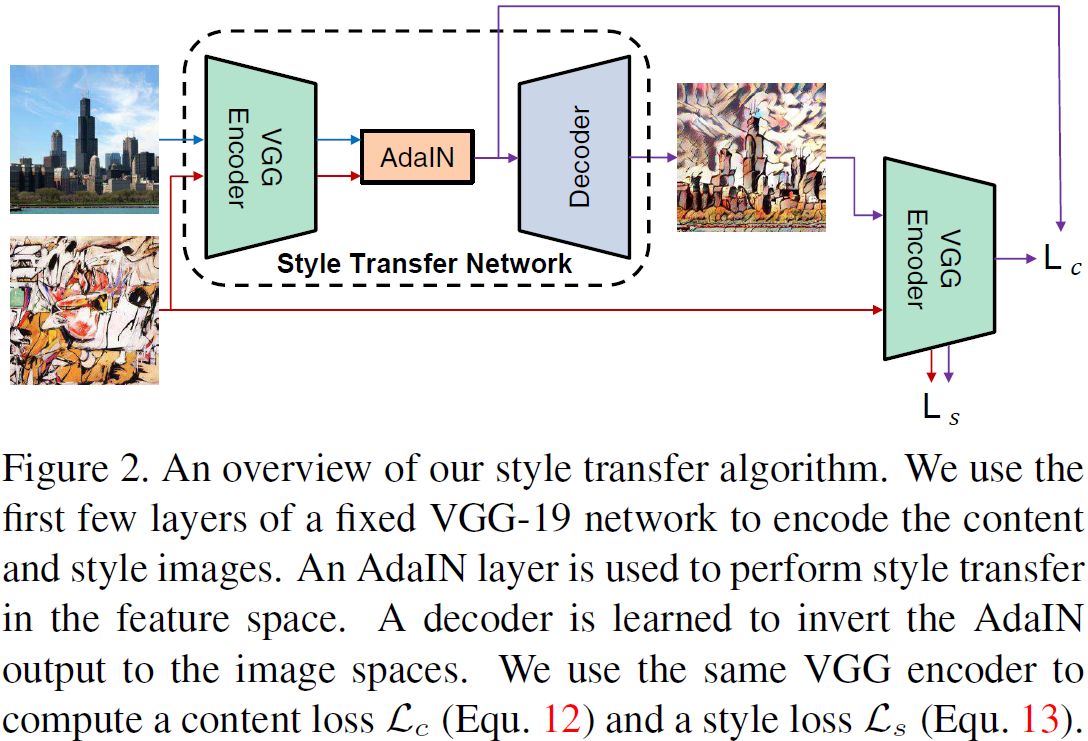
\includegraphics[width=0.71\textwidth]{img/1.png}
% \caption{首页}
% \label{fig:home}
% \end{figure}

用户在登入后,首页会显示用户昵称、头像等信息,并且可以跳转至用户个人主页、收藏、安全设置等页面,如图 \ref{fig:home-login} 所示。

% \begin{figure}[H]
% \centering
% 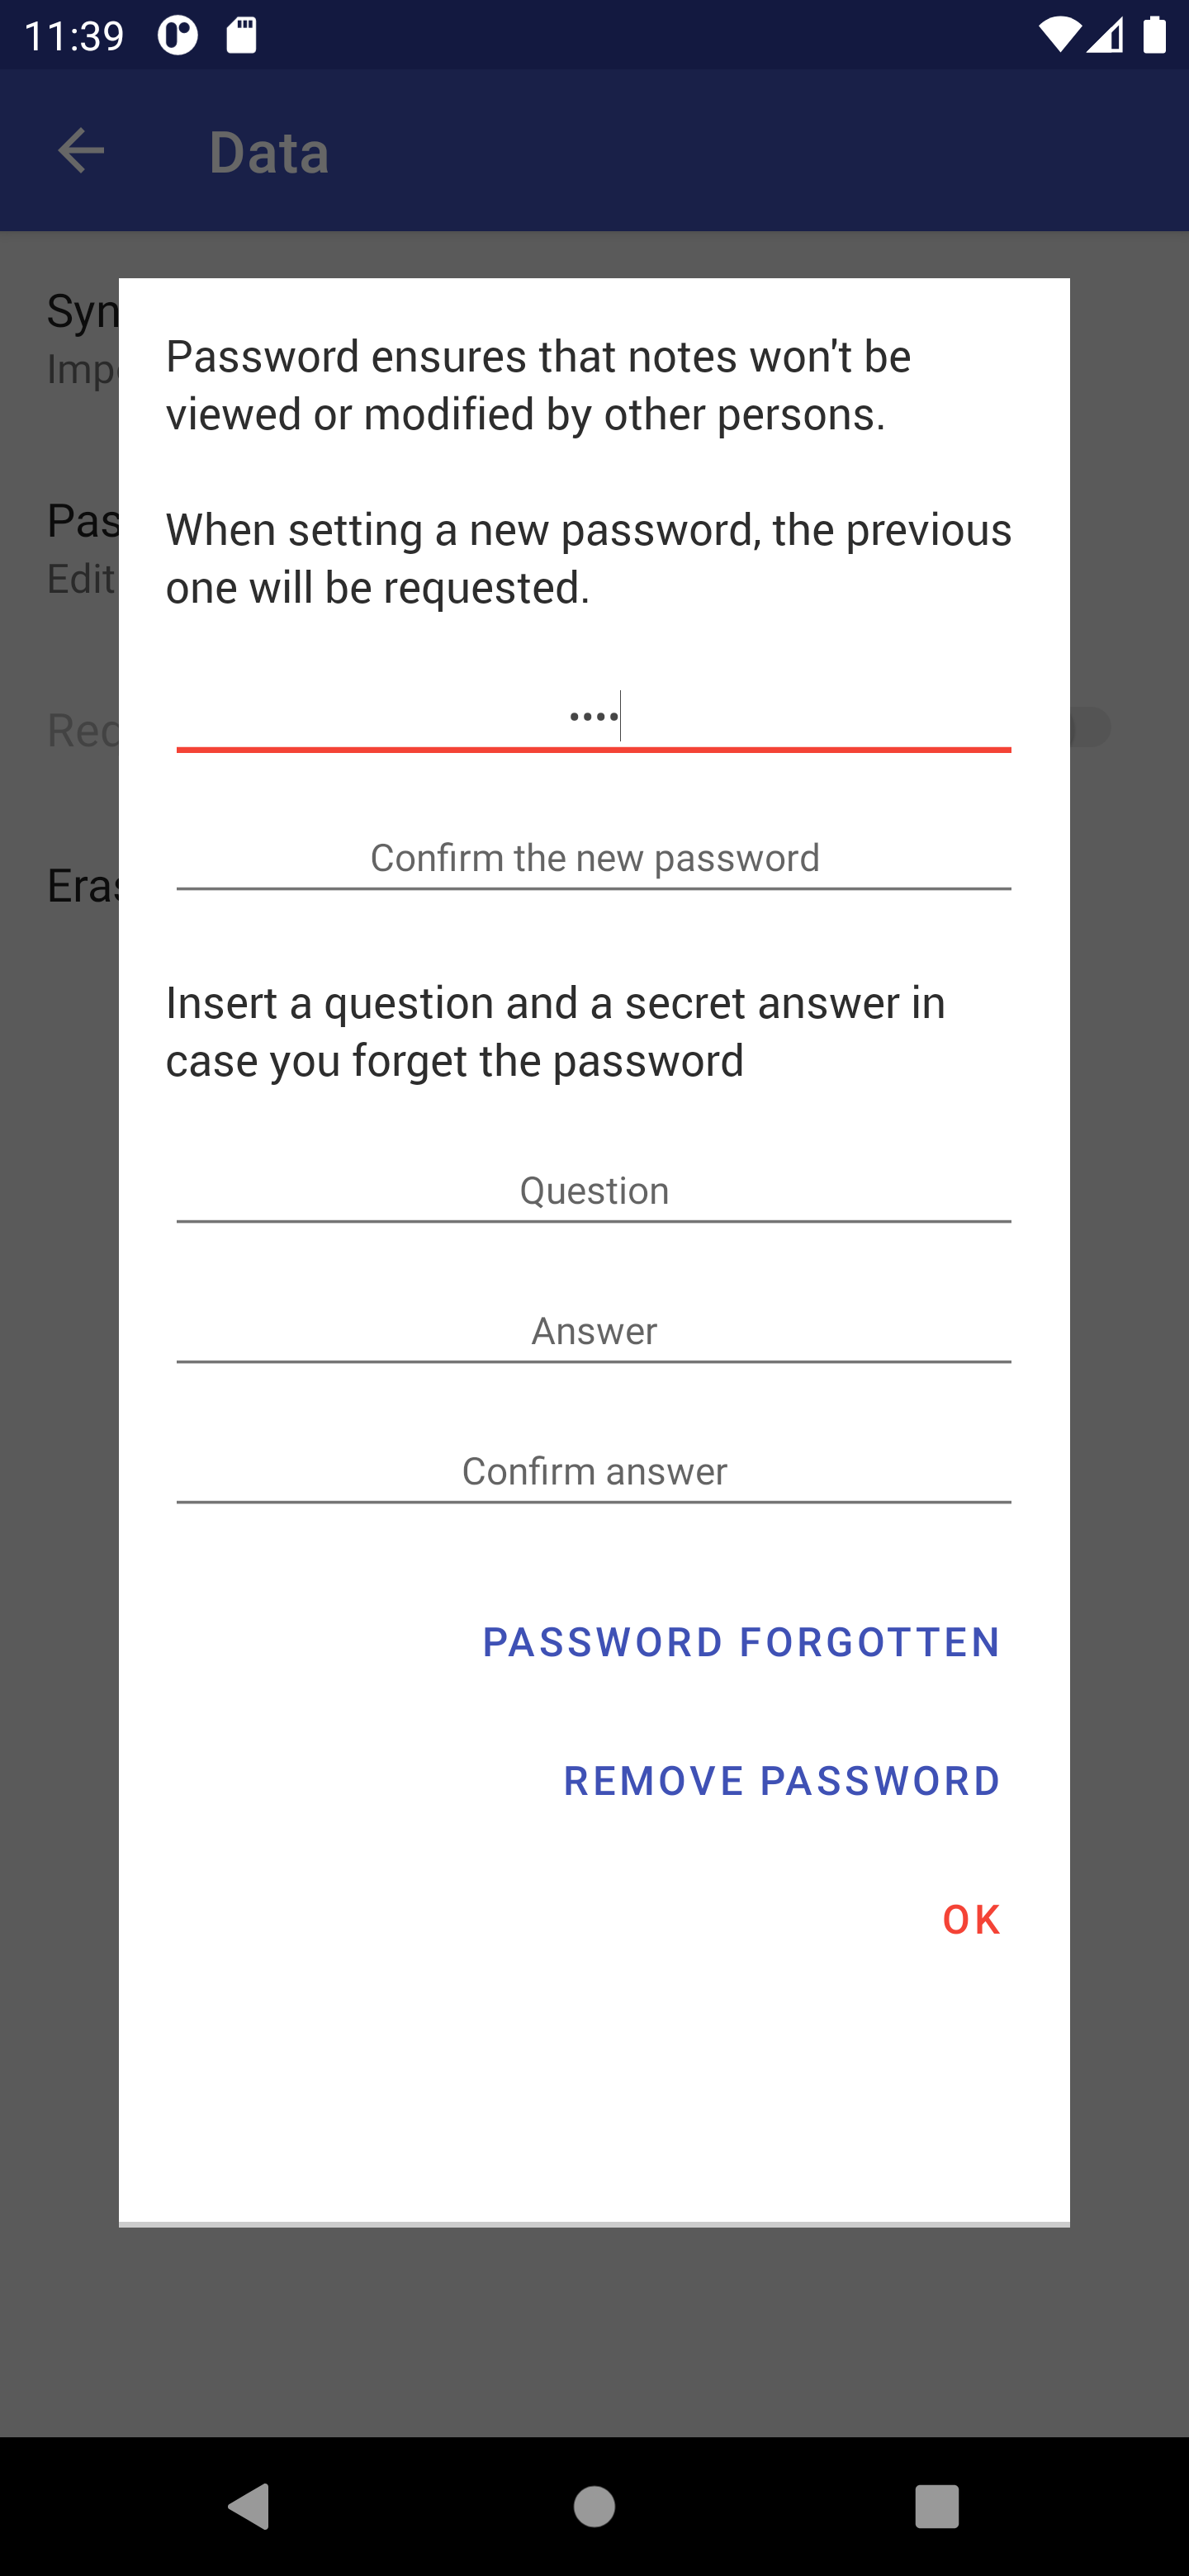
\includegraphics[width=0.71\textwidth]{img/2.png}
% \caption{首页(登录后)}
% \label{fig:home-login}
% \end{figure}

\section{搜索页}

用户在任意界面都可以进行搜索,搜索结果会显示在搜索页。搜索页包含搜索框、高级搜索、研究方向搜索等功能,用户可以对搜索结果进行排序,或对搜索结果进行筛选,如图 \ref{fig:search} 所示。

% \begin{figure}[H]
% \centering
% 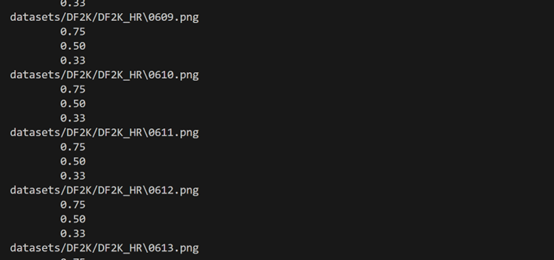
\includegraphics[width=0.9\textwidth]{img/3.png}
% \caption{搜索页}
% \label{fig:search}
% \end{figure}

\section{文献详情页}

用户点击文献,将跳转至文献页。用户可以查看文献的详细信息,包括标题、作者、摘要、发布时间、期刊等信息。用户可以查看文献的引用信息,包括引用与被引用,直接引用和间接引用。用户也可以跳转到文献全文所在的网址。如图 \ref{fig:detail} 所示。

% \begin{figure}[H]
% \centering
% 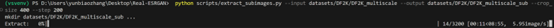
\includegraphics[width=0.9\textwidth]{img/4.png}
% \caption{文献详情页}
% \label{fig:detail}
% \end{figure}

用户点击摘要、期刊、作者等栏目,可以展开查看更多相关信息,如图 \ref{fig:detail-more} 所示。

% \begin{figure}[H]
% \centering
% 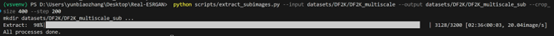
\includegraphics[width=0.9\textwidth]{img/5.png}
% \caption{文献详情页(更多信息)}
% \label{fig:detail-more}
% \end{figure}

\section{注册与登录页}

用户在任意界面点击注册,将跳转至注册页。用户在注册页输入邮箱,通过验证码认证后,设置密码完成注册,如图 \ref{fig:register} 所示。

% \begin{figure}[H]
% \centering
% 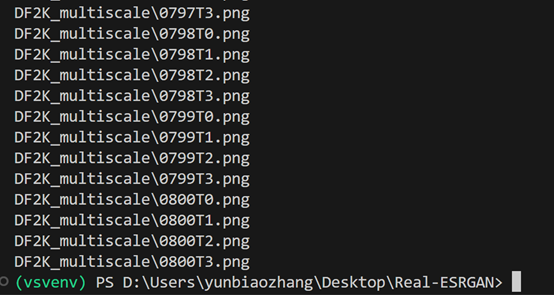
\includegraphics[width=0.9\textwidth]{img/7.png}
% \caption{注册页}
% \label{fig:register}
% \end{figure}

用户在任意界面点击登录,将跳转至登录页。用户在登录页输入邮箱和密码,完成登录,如图 \ref{fig:login} 所示。

% \begin{figure}[H]
% \centering
% 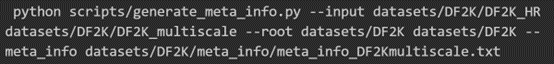
\includegraphics[width=0.9\textwidth]{img/6.png}
% \caption{登录页}
% \label{fig:login}
% \end{figure}

\section{用户页面}

用户在任意界面点击用户信息按钮,将跳转至用户信息页面。在用户信息页面,用户可以查看和修改自己的个人信息,包括昵称、头像、座右铭、学院等信息。用户也可以修改个人信息偏好,如是否存储浏览历史等。如图 \ref{fig:user-info} 所示。

% \begin{figure}[H]
% \centering
% 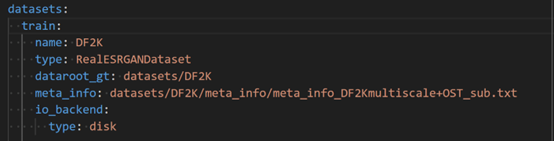
\includegraphics[width=0.9\textwidth]{img/8.png}
% \caption{用户信息}
% \label{fig:user-info}
% \end{figure}

用户点击收藏按钮,将跳转至收藏页面。在收藏页面,用户可以查看自己收藏的文献,如图 \ref{fig:collect} 所示。

% \begin{figure}[H]
% \centering
% 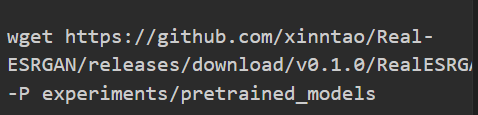
\includegraphics[width=0.9\textwidth]{img/9.png}
% \caption{收藏}
% \label{fig:collect}
% \end{figure}

用户点击安全设置按钮,将跳转至安全设置页面。在安全设置页面,用户可以修改密码,如图 \ref{fig:security} 所示。

% \begin{figure}[H]
% \centering
% 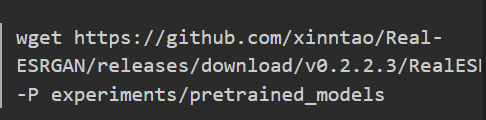
\includegraphics[width=0.9\textwidth]{img/10.png}
% \caption{安全设置}
% \label{fig:security}
% \end{figure}

\chapter{\texttt{SQL}}
\label{sec:sql}

在此部分,我们将展示部分 \texttt{SQL} 语句,用于实现系统相关功能。

由于数据量较大,我们考虑在查询时应该使用分页查询,以减少查询时间。我们使用 \texttt{LIMIT} 和 \texttt{OFFSET} 关键字来实现分页查询,例如,\texttt{LIMIT n OFFSET m}或\texttt{LIMIT m, n} 表示从第 $m+1$ 行开始取 $n$ 行数据。\textbf{为了使报告中的 \texttt{SQL} 语句更加简洁,我们在此省略了分页查询的部分}。

在下面的代码中,\texttt{SQL} 语句中的 \texttt{?} 表示占位符,用于接收用户输入的参数。

\section{用户相关功能}

根据用户邮箱和密码进行注册:

\begin{lstlisting}[language=SQL]
INSERT INTO `user` (`email`, `password`) VALUES (?, ?);
\end{lstlisting}

根据邮箱查询用户:

\begin{lstlisting}[language=SQL]
SELECT * FROM `user` WHERE email = ?;
\end{lstlisting}

根据用户传入的新密码和用户的id来修改密码:

\begin{lstlisting}[language=SQL]
UPDATE `user` SET `password` = ? WHERE `id` = ?;
\end{lstlisting}

根据用户传入修改信息来对原信息进行修改:

\begin{lstlisting}[language=SQL]
UPDATE `user` SET `nickname` = ?, `avatar` = ?, `motto` = ?, 
  `collage` = ?, `subscribe_email` = ? `save_history` = ? 
  WHERE `id` = ?;
\end{lstlisting}

根据用户的ID和期刊的名称实现用户订阅感兴趣的期刊:

\begin{lstlisting}[language=SQL]
INSERT INTO `subscribe` VALUES(?,?);
\end{lstlisting}

根据用户的ID和文献的ID用户实现收藏感兴趣的文献:

\begin{lstlisting}[language=SQL]
INSERT INTO `collect` VALUES(?,?); 
\end{lstlisting}

根据用户的ID来实现查看用户的浏览历史:

\begin{lstlisting}[language=SQL]
SELECT * FROM `history` WHERE `user_id` = ?;
\end{lstlisting}

\textbf{定时任务}——删除过期的浏览历史\footnote{需要安装\texttt{pg\_cron}插件}:

\begin{lstlisting}[language=sql]
CREATE EXTENSION pg_cron;
SELECT cron.schedule(
  'daily_clean_history',  
  '0 0 * * *',
  $$
  DELETE FROM history
  WHERE time < NOW() - INTERVAL '1 month';
  $$
);
\end{lstlisting}


\section{搜索相关功能}

根据作者姓名(模糊)搜索作者信息:

\begin{lstlisting}[language=sql]
SELECT * FROM `author` WHERE `name` LIKE "%?%";
\end{lstlisting}

根据作者姓名(模糊)搜索其撰写的文献:

\begin{lstlisting}[language=sql]
SELECT `author_name`, `id`, `title`, `abstract`,`doi`,
  `license`, `publish_time`, `url` 
FROM `write` JOIN `article` 
ON `article_id` = `id` 
WHERE `author_name` LIKE "%?%";
\end{lstlisting}

根据文献标题(模糊)搜索文献:

\begin{lstlisting}[language=sql]
SELECT `id`, `title`, `abstract`, `doi`, `license`
FROM (
  SELECT * 
  FROM `article`
  WHERE `title` LIKE "%?%"
) AS `art`
JOIN `publish` ON `id`=`publish`.`article_id`
JOIN `write` ON `id`=`write`.`article_id`;
\end{lstlisting}

根据期刊名模糊搜索期刊:

\begin{lstlisting}[language=sql]
SELECT * 
FROM `journal` 
WHERE `journal`.`name` LIKE "%?%";
\end{lstlisting}

根据期刊名模糊搜索该期刊刊登的文章:
\begin{lstlisting}[language=sql]
SELECT * 
FROM `publish` JOIN `article` ON `article_id` = `id`
WHERE `journal_name` LIKE "%?%";
\end{lstlisting}

根据研究方向、研究对象和研究问题搜索文献:
\begin{lstlisting}[language=sql]
SELECT `id`, `title`, `abstract`, `doi`, `license`, 
  `publish_time`, `url`, `journal_name`
FROM (
  SELECT * 
  FROM `article`
  WHERE `study_type` LIKE "%?%"
  OR `addressed_population` LIKE "%?%"
  OR `challenge` LIKE "%?%"
  OR `focus` LIKE "%?%"
) AS `art`
JOIN `publish` ON `id`=`publish`.`article_id`
JOIN `write` ON `id`=`write`.`article_id`;
\end{lstlisting}



\section{文献相关功能}

根据文献ID查询文献的详细信息:

\begin{lstlisting}[language=sql]
SELECT `id`,`title`,`abstract`,`doi`,`license`,`publish_time`,`url`,`study_type`,
`addressed_population`,`challenge`,`focus`,`journal_name`,`volume`,`pages`
FROM `article` JOIN `publish` ON `id`=`article_id`
WHERE `id` = ?;
\end{lstlisting}

根据文献ID查询作者:

\begin{lstlisting}[language=sql]
SELECT `write`.author_name
FROM `article` JOIN `write` ON article_id = `id`
WHERE `id`= ?;
\end{lstlisting}

\textbf{函数}——插入被引用的文献:

\begin{lstlisting}[language=sql]
CREATE OR REPLACE FUNCTION "public"."insert_cited_art"(
  "aid" varchar, 
  "in_title" varchar, 
  "in_doi" varchar, 
  "in_publish_time" timestamptz, 
  "in_journal" varchar, 
  "in_volume" varchar, 
  "in_pages" varchar, 
  "authors" varchar
)
RETURNS "pg_catalog"."void" AS $BODY$
DECLARE
  cnt INT;
  current_author VARCHAR;
  position INT;
BEGIN
  SELECT COUNT(*) INTO cnt FROM article WHERE title = in_title;
  IF cnt = 0 THEN  
    BEGIN
      INSERT INTO article(id, title, doi, publish_time) VALUES(aid, in_title, in_doi, in_publish_time)
      ON CONFLICT (id) DO NOTHING;
    EXCEPTION WHEN unique_violation THEN   
    END;
    position := 1;
    WHILE POSITION(';' IN authors) > 0 LOOP
      current_author := SUBSTRING(authors, 1, POSITION(';' IN authors) - 1);
      BEGIN
        INSERT INTO author(name) VALUES(current_author)
        ON CONFLICT (name) DO NOTHING;
      EXCEPTION WHEN unique_violation THEN 
      END;
      BEGIN
        INSERT INTO write(author_name, article_id) VALUES(current_author, aid)
        ON CONFLICT (author_name, article_id) DO NOTHING;
      EXCEPTION WHEN unique_violation THEN 
      END;
      authors := SUBSTRING(authors, POSITION(';' IN authors) + 1);
    END LOOP;
    current_author := authors;
    BEGIN
      INSERT INTO author(name) VALUES(current_author)
      ON CONFLICT (name) DO NOTHING;
    EXCEPTION WHEN unique_violation THEN  
    END;
    BEGIN
      INSERT INTO write(author_name, article_id) VALUES(current_author, aid)
      ON CONFLICT (author_name, article_id) DO NOTHING;
    EXCEPTION WHEN unique_violation THEN  
    END;
    BEGIN
      INSERT INTO journal(name) VALUES(in_journal)
      ON CONFLICT (name) DO NOTHING;
    EXCEPTION WHEN unique_violation THEN    
    END;
    BEGIN
      INSERT INTO publish(journal_name, article_id, volume, pages) VALUES(in_journal, aid, in_volume, in_pages)
      ON CONFLICT (journal_name, article_id) DO NOTHING;
    EXCEPTION WHEN unique_violation THEN  
    END;
  END IF;
END;
$BODY$
  LANGUAGE plpgsql VOLATILE
  COST 100
\end{lstlisting}

\textbf{函数}——插入扩展文章:

\begin{lstlisting}[language=sql]
CREATE OR REPLACE FUNCTION "public"."insert_extend_art"(
  "aid" varchar, 
  "in_title" varchar, 
  "in_publish_time" timestamptz, 
  "in_url" varchar, 
  "in_study_type" varchar, 
  "in_addressed_population" varchar, 
  "in_challenge" varchar, 
  "in_focus" varchar, 
  "in_journal" varchar
)
RETURNS "pg_catalog"."void" AS $BODY$
DECLARE
  cnt INT;
BEGIN
  SELECT COUNT(*) INTO cnt FROM article WHERE title = in_title;
  IF cnt = 0 THEN
    INSERT INTO article(id, title, publish_time, url, study_type, addressed_population, challenge, focus)
    VALUES(aid, in_title, in_publish_time, in_url, in_study_type, in_addressed_population, in_challenge, in_focus)
    ON CONFLICT (id) DO NOTHING;
    INSERT INTO journal(name) VALUES (in_journal)
    ON CONFLICT (name) DO NOTHING;
    INSERT INTO publish(journal_name, article_id, volume, pages)
    VALUES(in_journal, aid, NULL, NULL)
    ON CONFLICT (journal_name, article_id) DO NOTHING;
  END IF;
END;
$BODY$
  LANGUAGE plpgsql VOLATILE
  COST 100
\end{lstlisting}

\textbf{递归查询}——查询文献的直接引用和间接引用:

\begin{lstlisting}[language=sql]
WITH RECURSIVE `c` AS (
  SELECT `citing_id`, `cited_id`, 0 AS `flag` FROM `cite`
  WHERE `citing_id` = ?
  UNION
  SELECT `citing_id`, `id`, 1 AS `flag` FROM `c` JOIN `article`
  ON `c`.`cited_id` = `article`.`id`
) 
SELECT * FROM `c`;
\end{lstlisting}

\chapter{测试与性能}
\label{sec:performance}

\section{测试语句}

在导入了全部数据集后,我们选取了18条\texttt{SQL}语句进行测试,如下所示:

\begin{enumerate}[label=\textbf{\arabic*}]
  \item 根据邮箱和密码以及用户昵称注册
  \begin{lstlisting}[language=sql]
INSERT INTO "user" ("id", nickname, email, "password") VALUES (0, 'test_name', 'test_email', '13456');
  \end{lstlisting}

  \item 根据邮箱查询用户:
  \begin{lstlisting}[language=sql]
SELECT * FROM "user" WHERE email = 'test_email';
  \end{lstlisting}

  \item 根据用户传入的新密码和用户的 id 来修改密码:
  \begin{lstlisting}[language=sql]
UPDATE "user" SET "password" = '456789' WHERE id = 0;
  \end{lstlisting}

  \item 根据用户传入修改信息来对原信息进行修改:
  \begin{lstlisting}[language=sql]
UPDATE "user"
SET nickname = 'test_name2', avatar = 'dsaw', motto = 'sadw',
  collage = 'col', subscribe_email = 'true', save_history = true
WHERE id = 0;
  \end{lstlisting}

  \item 根据用户的 ID 和期刊的名称实现用户订阅感兴趣的期刊:
  \begin{lstlisting}[language=sql]
INSERT INTO subscribe (user_id, journal_name) VALUES (0, 'Respir Res');
  \end{lstlisting}

  \item 根据用户的 ID 和文献的 ID 用户实现收藏感兴趣的文献:
  \begin{lstlisting}[language=sql]
INSERT INTO "collect" (user_id, article_id) VALUES (0, 'tn4ba9le');
  \end{lstlisting}

  \item 根据用户的 ID 来实现查看用户的浏览历史:
  \begin{lstlisting}[language=sql]
SELECT * FROM "history" WHERE user_id = 0;
  \end{lstlisting}

  \item 根据作者姓名(模糊)搜索作者信息:
  \begin{lstlisting}[language=sql]
SELECT * FROM author WHERE name LIKE '%' || 'aa' || '%';
  \end{lstlisting}

  \item 根据作者姓名(模糊)搜索其撰写的文献:
  \begin{lstlisting}[language=sql]
SELECT w.author_name, ar.id, ar.title, ar.abstract, ar.doi, ar.license, ar.publish_time, ar.url
FROM "write" w
JOIN article ar ON w.article_id = ar.id
WHERE w.author_name LIKE '%' || 'aa' || '%';
  \end{lstlisting}

  \item 根据文献标题(模糊)搜索文献:
  \begin{lstlisting}[language=sql]
SELECT ar.id, ar.title, ar.abstract, ar.doi, ar.license
FROM article ar
JOIN publish p ON ar.id = p.article_id
JOIN write w ON ar.id = w.article_id
WHERE ar.title LIKE '%' || 'aa' || '%';
  \end{lstlisting}

  \item 根据期刊名模糊搜索期刊:
  \begin{lstlisting}[language=sql]
SELECT *
FROM journal
WHERE name LIKE '%' || 'Res' || '%';
  \end{lstlisting}

  \item 根据期刊名模糊搜索该期刊刊登的文章:
  \begin{lstlisting}[language=sql]
SELECT ar.*
FROM publish p
JOIN article ar ON p.article_id = ar.id
WHERE p.journal_name LIKE '%' || 'aa' || '%';
  \end{lstlisting}

  \item 根据研究方向、研究对象和研究问题搜索文献:
  \begin{lstlisting}[language=sql]
SELECT ar.id, w.author_name, ar.title, ar.abstract, ar.doi, ar.license, 
  ar.publish_time, ar.url, p.journal_name
FROM article ar
JOIN publish p ON ar.id = p.article_id
JOIN write w ON ar.id = w.article_id
WHERE ar.study_type LIKE '%' || 'testst' || '%'
  OR ar.addressed_population LIKE '%' || 'testadd' || '%'
  OR ar.challenge LIKE '%' || 'testcl' || '%'
  OR ar.focus LIKE '%' || 'testfo' || '%';
  \end{lstlisting}

  \item 根据文献 ID 查询文献的详细信息:
  \begin{lstlisting}[language=sql]
SELECT ar.id, ar.title, ar.abstract, ar.doi, ar.license, ar.publish_time, ar.url,
  ar.study_type, ar.addressed_population, ar.challenge, ar.focus,
  p.journal_name, p.volume, p.pages
FROM article ar
JOIN publish p ON ar.id = p.article_id
WHERE ar.id = 'tn4ba9le';
  \end{lstlisting}

  \item 根据文献 ID 查询作者:
  \begin{lstlisting}[language=sql]
SELECT w.author_name
FROM article ar
JOIN write w ON ar.id = w.article_id
WHERE ar.id = 'tn4ba9le';
  \end{lstlisting}

  \item 查询文献的直接引用和间接引用:
  \begin{lstlisting}[language=sql]
WITH RECURSIVE c AS (
  SELECT citing_id, cited_id, 0 AS flag
  FROM cite
  UNION ALL
  SELECT cite.citing_id, cite.cited_id, 1 AS flag
  FROM c
  JOIN cite ON c.cited_id = cite.citing_id
)
SELECT * FROM c;
  \end{lstlisting}

  \item 测试函数\texttt{insert\_cited\_art}:
  \begin{lstlisting}[language=sql]
SELECT insert_cited_art('test_id', 'test_title', 'test_doi', '2024/6/5', 'test_journal', 'test_volume', 'test_in_pages', '0;1');
  \end{lstlisting}

  \item 测试函数\texttt{insert\_extend\_art}:
  \begin{lstlisting}[language=sql]
SELECT insert_extend_art('test_id', 't_title', '2024/6/5', 't_url', 't_type', 't_addr', 't_cha', 't_focus', 't_journal');
  \end{lstlisting}
\end{enumerate}

\section{测试结果}

我们使用 \texttt{EXPALIN} 命令来查看每条 \texttt{SQL} 语句的执行计划,以评估其性能。我们将测试结果汇总如表 \ref{tab:performance} 所示。

\begin{table}[H]
  \caption{性能测试结果}
  \centering
\label{tab:performance}
\begin{tabular}{cc}
\toprule
\textbf{序号} &  \textbf{执行时间/ms} \\ 
\midrule
1	&34 \\
2	&32 \\
3	&32 \\
4	&32 \\
5	&34 \\
6	&32 \\
7	&31 \\
8	&389 \\
9	&1028 \\
10&	2063 \\
11&	441 \\
12&	362 \\
13&	526 \\
14&	158 \\
15&	505 \\
16&	36 \\
17&	270.68 \\
18&	270.865 \\
\bottomrule
\end{tabular}
\end{table}

\section{性能分析与优化}

从表 \ref{tab:performance} 中可以看出,大部分 \texttt{SQL} 语句的执行时间都在 1000ms 以内,性能较好。但是,有两条 \texttt{SQL} 语句的执行时间较长,分别为 2063ms 和 1028ms。这是因为这两条 \texttt{SQL} 语句中包含了多个表的连接查询,导致了性能下降。我们可以通过增加索引来提高性能。

在增加了索引后,我们再次进行了测试,结果如表 \ref{tab:performance2} 所示。

\begin{longtable}[c]{cc}
  \caption{性能测试结果(优化后)} \label{tab:performance2} \\
\toprule
\textbf{序号} &  \textbf{执行时间/ms} \\
\midrule
\endfirsthead

\caption[]{性能测试结果(优化后) (续表)} \\
\toprule
\textbf{序号} &  \textbf{执行时间/ms} \\
\midrule
\endhead

\midrule
\multicolumn{2}{r}{续下页}
\endfoot

\bottomrule
\endlastfoot

1	&36 \\
2	&34 \\
3	&37 \\
4	&36 \\
5	&38 \\
6	&36 \\
7	&36 \\
8	&66 \\
9	&956 \\
10&	639 \\
11&	350 \\
12&	118 \\
13&	417 \\
14&	39 \\
15&	35 \\
16&	37 \\
17&	3.27 \\
18&	0.824 \\
\end{longtable}

从表 \ref{tab:performance2} 中可以看出,经过优化后,性能有一定的提升。其中,第 10 条 \texttt{SQL} 语句的执行时间从 2063ms 降低到 639ms。这说明增加索引对性能有一定的提升作用。改进后的性能已经可以满足系统的需求。

两次测试的对比结果如下图所示。

% \begin{figure}[H]
%   \centering
%   \includegraphics[width=0.8\textwidth]{img/time.png}
%   \caption{性能测试结果对比}
%   \label{fig:performance}
% \end{figure}



\newpage

\appendix

\chapter{所附代码文件概述}
\label{appendix:code}

随本报告所附代码文件结构如下:

% \begin{figure}[H]
%   \dirtree{%
%       .1 process\_data.
%       .2 archive/\DTcomment{图 \ref{fig:dataset} 所示的数据集}.
%       .2 output/.
%       .3 deduplicated/\DTcomment{去重后的数据}.
%       .2 article.py\DTcomment{文献所包含的类}.
%       .2 main.py\DTcomment{主程序}.
%       .2 requirements.txt\DTcomment{依赖}.
%   }
%   \caption{所附代码文件结构}
%   \label{fig:processData}
% \end{figure}

使用方法:



\begin{enumerate}
  \item 下载数据集
  \item 安装依赖:
\begin{lstlisting}[language=bash]
pip install -r requirements.txt
\end{lstlisting}
  \item 运行\texttt{main.py}。
\begin{lstlisting}[language=bash]
python main.py
\end{lstlisting}
\end{enumerate}

\newpage

\chapter{本报告在Milestone 1报告基础上的变化}

\begin{enumerate}
    \item 在 \ref{sec:overviewOfDatabaseDesign} 节中,我们更换了使用的数据库管理系统,从MySQL变为PostgreSQL。
    \item 在 \ref{sec:dataProcessing} 节中,我们更改了数据处理的方式,先将数据处理后存储到本地文件中,再使用数据库的 \texttt{COPY} 命令批量插入数据,以提高性能。
    \item 在 \ref{sec:sql} 章中,我们修改了函数/存储过程的代码和部分 \texttt{SQL} 语句,以符合PostgreSQL的语法。
    \item 增加了第 \ref{sec:performance} 章,对系统的性能进行了测试和分析。
    \item 增加了附录\ref{appendix:code},展示了所附代码文件的结构和使用方法。
\end{enumerate}

\end{document}